\subsection{Modulation}
\begin{enumerate}[label=\thesubsection.\arabic*.,ref=\thesubsection.\theenumi]
\numberwithin{equation}{enumi}
\numberwithin{figure}{enumi}



\item See Fig.\ref{fig:ee18btech11041_fig1} for the constellation diagram.  The transmitted symbol set is given by 
\begin{align}
\vec{s}_m = \myvec{\cos \frac{2m\pi}{8}\\ \sin \frac{2m\pi}{8}}, \quad m \in \cbrak{0, 1, \dots, 3}.
%\textbf{y = s + n}
\end{align}
%
The numerical values for $\vec{s}_m$ are listed in Table \ref{table:ee18btech11041_table1}

\begin{figure}[!ht]
                \resizebox{\columnwidth}{!}{
\begin{tikzpicture}

\draw[<->,thick] (-4,0)--(4,0) node[right]{$\phi_1$};
\draw[<->,thick] (0,-4)--(0,4) node[above]{$\phi_2$};

\filldraw[black] (2.5,0) circle (2pt) node[below] {$s_0$} ;
\filldraw[black] (0,2.5) circle (2pt) node[left] {$s_1$} ;
\filldraw[black] (-2.5,0) circle (2pt) node[below] {$s_2$} ;
\filldraw[black] (0,-2.5) circle (2pt) node[left] {$s_3$} ;

\end{tikzpicture}
}

\caption{constellation diagram}
\label{fig:ee18btech11041_fig1}
\end{figure}

%
\item See Table \ref{table:ee18btech11041_table1} for the encoding scheme.


\begin{table}[!ht]
\centering
\input{./tables/ee18btech11041_table1.tex}
\caption{}
\label{table:ee18btech11041_table1}
\end{table}


\end{enumerate}
\subsection{Demodulation}
\begin{enumerate}[label=\thesubsection.\arabic*.,ref=\thesubsection.\theenumi]
\item The received symbol is then obtained as
\begin{align}
\vec{y} = \sqrt{E_s}\vec{s} + \vec{n}
\end{align}
%
where $E_s$ is the symbol energy and 

\begin{align}
\vec{n} &\sim \mathcal{N}\brak{\vec{0},\frac{N_0}{2}\vec{I}}
\\
\vec{s} &\in \cbrak{\vec{s}_m}_{m = 0}^{3}
\end{align}
\item The decision rule is given by Fig.\ref{fig:ee18btech11041_fig2} and can be expressed as

\begin{figure}[!ht]
                \resizebox{\columnwidth}{!}{
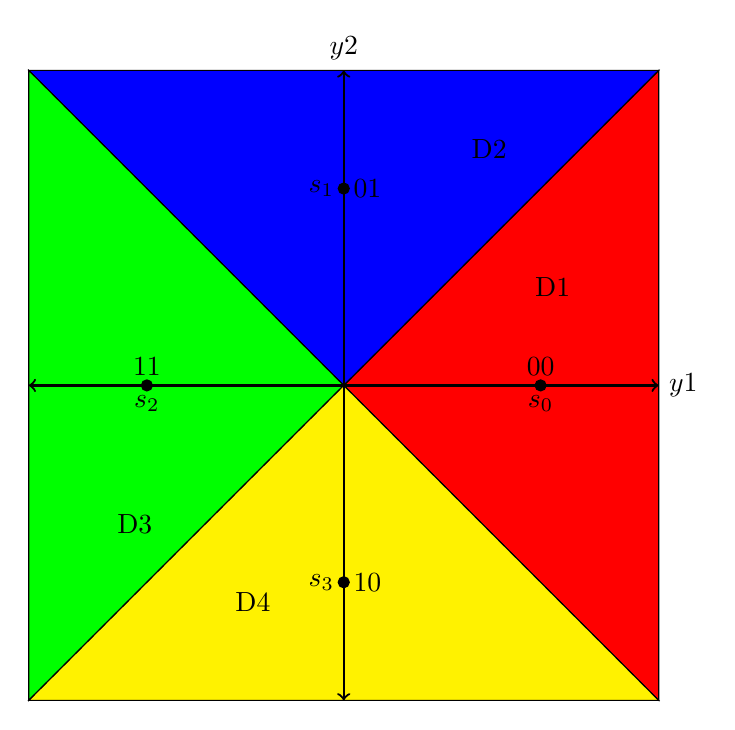
\begin{tikzpicture}


\draw[fill=red]  (0,0) -- (4,4) -- (4,-4)  -- cycle;

\draw[fill=blue]  (0,0) -- (4,4) -- (-4,4)  -- cycle;
\draw[fill=green]  (0,0) -- (-4,4) -- (-4,-4)  -- cycle;
\draw[fill=yellow]  (0,0) -- (-4,-4) -- (4,-4)  -- cycle;



\draw[<->,thick] (-4,0)--(4,0) node[right]{$y1$};
\draw[<->,thick] (0,-4)--(0,4) node[above]{$y2$};
\draw [dashed]   (-4,-4)--(4,4);
\draw [dashed]   (-4,4)--(4,-4);

\filldraw[black] (2.5,0) circle (2pt) node[below] {$s_0$} node[above] {00};
\filldraw[black] (0,2.5) circle (2pt) node[left] {$s_1$} node[right] {01};
\filldraw[black] (-2.5,0) circle (2pt) node[below] {$s_2$} node[above] {11};
\filldraw[black] (0,-2.5) circle (2pt) node[left] {$s_3$} node [right] {10} ;


\foreach \coordinate/\label/\pos in {{(3,1)/D1/above left},{(1.5,3)/D2/right},{(-3,-2)/D3/above right},{(-1.5,-3)/D4/above right}} \node[\pos] at \coordinate {\label};

\end{tikzpicture}
}


\caption{decision regions}
\label{fig:ee18btech11041_fig2}	
\end{figure}

\textbf{\underline{Minimum distance Criterion}:}
\begin{align}
    \hat{s} = min \norm{\textbf{y} - \textbf{s}}
    \label{eq:ee18btech11041_eq1}
\end{align}

From eq.\ref{eq:ee18btech11041_eq1},\textbf{$s_{0}$} is chosen if

\begin{align}
    \norm{\vec{y}-\vec{s}_0}^2 < \norm{\vec{y}-\vec{s}_1}^2
\end{align}
\begin{align}
    \norm{\vec{y}-\vec{s}_0}^2 < \norm{\vec{y}-\vec{s}_2}^2
\end{align}
\begin{align}
    \norm{\vec{y}-\vec{s}_0}^2 < \norm{\vec{y}-\vec{s}_3}^2
\end{align}

The above conditions can be simplified to obtain the region


\begin{align}
    (\vec{s}_0-\vec{s}_1)^T\vec{y}>0
\end{align}
\begin{align}
    (\vec{s}_0-\vec{s}_2)^T\vec{y}>0
\end{align}
\begin{align}
    (\vec{s}_0-\vec{s}_3)^T\vec{y}>0
\end{align}

Substituting the values of $s_{0}$,$s_{1}$,....$s_{7}$ in the above


\begin{align}
\myvec{1 \\ -1}^T\vec{y}&> 0
\\
\myvec{1\\ 0}^T\vec{y}&> 0
\\
\myvec{1 \\ 1}\vec{y}^T &> 0
\end{align}
\\
yielding $\abs{y_2}<$ y1  i.e D1 region (red) is detected at the receiver.
\\
Similarly, from eq.\ref{eq:ee18btech11041_eq1}
\\
For detecting $s_1$, $y_1>-y_2$ and $y_1<y_2$ i.e D2 region (blue) is detected at the receiver.
\\
For detecting $s_2$,  $y_1<-y_2$ and $y_1<y_2$ i.e D3 region (green) is detected at the receiver.
\\
For detecting $s_3$, $y_1<-y_2$ and $y_1>y_2$ i.e D4 region (yellow) is detected at the receiver.




\begin{table}[!ht]
\centering
\input{./tables/ee18btech11041_table2.tex}
\caption{}
\label{table:ee18btech11041_table2}
\end{table}



\item The following code has simulation of QPSk.
\begin{lstlisting}
 codes/qpsk.py
\end{lstlisting}


\begin{figure}[!h]
    \includegraphics[width=\columnwidth]{./figs/ee18btech11041_fig3.eps}
    \caption{Result from Simulation}
    \label{fig:ee18btech11041_fig3}
\end{figure}



\end{enumerate}
